\documentclass[9pt,twocolumn,twoside]{gsajnl}
% Use the documentclass option 'lineno' to view line numbers

\articletype{inv} % article type
% {inv} Investigation 
% {gs} Genomic Selection
% {goi} Genetics of Immunity 
% {gos} Genetics of Sex 
% {mp} Multiparental Populations

\title{Kidney renal clear cell carcinoma expression analyse}

\author[$\ast$1]{Bofill A,}
\author[$\ast$1]{Castillo S,}
\author[$\ast$1]{Pérez A}


\affil[$\ast$]{Msc in Bioinformatics for Health Sciences, Pompeu Fabra University}

\keywords{Kidney; Carcinoma; Bioconductor; ASS. Sergio Castillo ...}

\runningtitle{GENETICS Journal Template on Overleaf} % For use in the footer 

\correspondingauthor{Corresponding Author}

\begin{abstract}
The abstract should be written for people who may not read the entire paper, so it must stand on its own. The impression it makes usually determines whether the reader will go on to read the article, so the abstract must be engaging, clear, and concise. In addition, the abstract may be the only part of the article that is indexed in databases, so it must accurately reflect the content of the article. A well-written abstract is the  most effective way to reach intended readers, leading to more robust search, retrieval, and usage of the article. 

\end{abstract}
\setboolean{displaycopyright}{true}
\begin{document}
\maketitle
\thispagestyle{firststyle}
\marginmark
\firstpagefootnote
\correspondingauthoraffiliation{Msc in Bioinformatics for Health Sciences, Pompeu Fabra University. adria.perez06@estudiant.upf.edu}
\vspace{-11pt}%

\section*{Your Abstract}

In addition to the guidelines provided in the example abstract above, your abstract should:
\begin{itemize}
\item provide a synopsis of the entire article;
\item begin with the broad context of the study, followed by specific background for the study;
\item describe the purpose, methods and procedures, core findings and results, and conclusions of the study;
\item emphasize new or important aspects of the research;
\item engage the broad readership of GENETICS and be understandable to a diverse audience (avoid using jargon);
\item be a single paragraph of less than 250 words;
\item contain the full name of the organism studied;
\item NOT contain citations or abbreviations.
\end{itemize}

\section*{Introduction}

For the introduction, authors should be mindful of the broad readership of the journal. The introduction should set the stage for the importance of the work to a generalist reader and draw the reader in to the specific study. The scope and impact of the work should be clearly stated. In individual organisms where a mutant is being studied, the rationale for the study of that mutant must be clear to a geneticist not studying that particular organism. Similarly, study of particular phenotypes should be justified broadly and not on the basis of interest for that organism alone. General background on the importance of the genetic pathway and/or phenotype should be provided in a single, well-reasoned paragraph near the beginning of the introduction.

Authors are encouraged to:

\begin{itemize}
\item cite the supporting literature completely rather than select a subset of citations;
\item provide important background citations, including relevant review papers (to help orient the non-specialist reader);
\item to cite similar work in other organisms.
\end{itemize}

\section*{Materials and Methods}

\subsection*{Sample filtering}
The kidney Renal Clear-Cell Carcinoma RNA-seq data used in this study has been extracted from The Cancer Genome Atlas \href{<http://cancergenome.nih.gov>}{TGCA}. The data initially comprised 542 tumours and 72 normal samples. Each one of the samples have a total of 20115 genes. We have applied several filters to reduce the data samples:
\begin{itemize}
\item \textit{ Library size filtering:} In order to obtain a more reliable data, we need to filter out the samples with a low sequencing depth (< 45 Millions per read). We obtain a filtered data of: 298 tumor and 48 normal samples.
\item \textit{Paired data filtering:} The next step is pairing the normal and tumor data. It allows the reduction of our set and to obtain a more accurate information. This filter results in 38 normal and 38 tumor samples.
\end{itemize}
We also need to apply filters to reduce the gene sets:
\begin{itemize}
\item \textit{ expression levels filter:} To filter out the genes with a low expression, we use a cut-off of 1 log Counts per Milions (logCPM). With this filter we reduce the number of genes from 20.115 to 11.742 genes.
Manuscripts submitted to GENETICS should contain a clear de- scription of the experimental design in sufficient detail so that the experimental analysis could be repeated by another scientist
\end{itemize}

\subsection*{Statistical and Data Analysis } 
Analyses has been performed with R. See more information about that in: \url{www.r-project.org}. All packages used in this Project could be viewed on the DONDEEEEEEEEEE.


It is important to indicate what statistical analysis has been performed; not just the name of the software and options selected, but the method and model applied. In the case of many genes being examined simultaneously, or many phenotypes, a multiple comparison correction should be used to control the type I error rate, or a rationale for not applying a correction must be provided. The type of correction applied should be clearly stated. It should also be clear whether the p-values reported are raw, or after correction. Corrected p-values are often appropriate, but raw p-values should be available in the supporting materials so that others may perform their own corrections. In large scale data exploration studies (e.g. genome wide expression studies) a clear and complete description of the replication structure must be provided. 

\subsection*{Data Availability}

At the end of the Materials and Methods section, include a statement on reagent and data availability. Please read the Data and Reagent Policy before writing the statement. Make sure to list the accession numbers or DOIs of any data you have placed in public repositories. List the file names and descriptions of any data you will upload as supplemental information. The statement should also include any applicable IRB numbers. You may include specifications for how to properly acknowledge or cite the data.

For example: Strains are available upon request. File S1 contains detailed descriptions of all supplemental files. File S2 contains SNP ID numbers and locations. File S3 contains genotypes for each individual. Sequence data are available at GenBank and the accession numbers are listed in File S3. Gene expression data are available at GEO with the accession number: GDS1234. Code used to generate the simulated data is provided in file S4. 


\section*{Results and Discussion}

The results and discussion should not be repetitive. The results section should give a factual presentation of the data and all tables and figures should be referenced; the discussion should not summarize the results but provide an interpretation of the results, and should clearly delineate between the findings of the particular study and the possible impact of those findings in a larger context. Authors are encouraged to cite recent work relevant to their interpretations. Present and discuss results only once, not in both the Results and Discussion sections. It is sometimes acceptable to combine results and discussion. The text should be as succinct as possible. Heed Strunk and White's dictum: "Omit needless words!"
\newpage

\section*{Additional guidelines}

\subsection*{Numbers} In the text, write out numbers nine or less except as part of a date, a fraction or decimal, a percentage, or a unit of measurement. Use Arabic numbers for those larger than nine, except as the first word of a sentence; however, try to avoid starting a sentence with such a number.

\subsection*{Units} Use abbreviations of the customary units of measurement only when they are preceded by a number: "3 min" but "several minutes". Write "percent" as one word, except when used with a number: "several percent" but "75\%." To indicate temperature in centigrade, use ° (for example, 37°); include a letter after the degree symbol only when some other scale is intended (for example, 45°K).

\subsection*{Nomenclature and Italicization} Italicize names of organisms even when  when the species is not indicated.  Italicize the first three letters of the names of restriction enzyme cleavage sites, as in HindIII. Write the names of strains in roman except when incorporating specific genotypic designations. Italicize genotype names and symbols, including all components of alleles, but not when the name of a gene is the same as the name of an enzyme. Do not use "+" to indicate wild type. Carefully distinguish between genotype (italicized) and phenotype (not italicized) in both the writing and the symbolism.

\section*{In-text Citations}

Add citations using the \verb|\citep{}| command, for example \citep{neher2013genealogies} or for multiple citations, \citep{neher2013genealogies, rodelsperger2014characterization}

\section*{Examples of Article Components}
\label{sec:examples}

The sections below show examples of different header levels, which you can use in the primary sections of the manuscript (Results, Discussion, etc.) to organize your content.

\section*{First level section header}

Use this level to group two or more closely related headings in a long article.

\subsection*{Second level section header}

Second level section text.

\subsubsection*{Third level section header:}

Third level section text. These headings may be numbered, but only when the numbers must be cited in the text. 

\section*{Figures and Tables}

Figures and Tables should be labelled and referenced in the standard way using the \verb|\label{}| and \verb|\ref{}| commands.

\subsection*{Sample Figure}

Figure \ref{fig:spectrum} shows an example figure.

\begin{figure}[htbp]
\centering
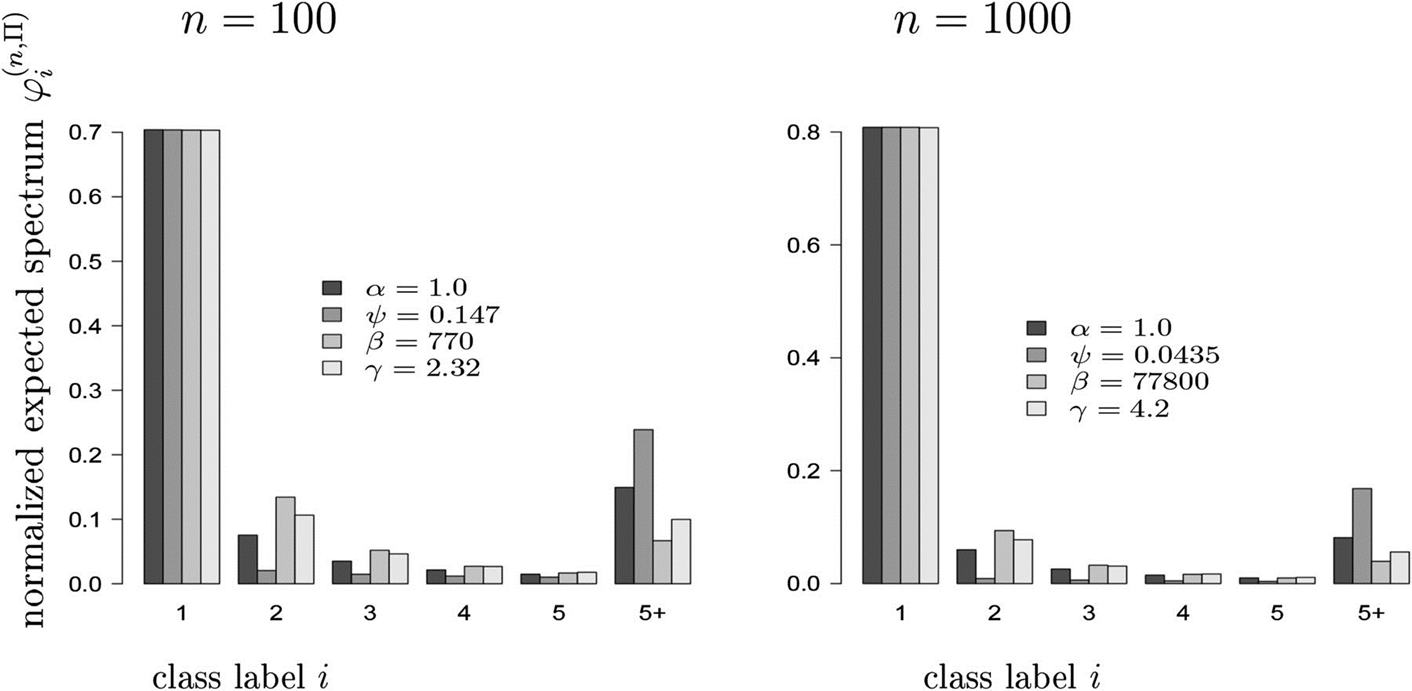
\includegraphics[width=\linewidth]{example-figure}
\caption{Example figure from \url{10.1534/genetics.114.173807}. Please include your figures in the manuscript for the review process. You can upload figures to Overleaf via the Project menu. Upon acceptance, we'll ask for your figure files to be uploaded in any of the following formats: TIFF (.tiff), JPEG (.jpg), Microsoft PowerPoint (.ppt), EPS (.eps), or Adobe Illustrator (.ai).  Images should be a minimum of 300 dpi in resolution and 500 dpi minimum if line art images.  RGB, CMYK, and Grayscale are all acceptable. Halftones should be high contrast with sharp detail, because some loss of detail and contrast is inevitable in the production process. Figures should be 10-20 cm in width and 1-25 cm in height. Graph axes must be exactly perpendicular and all lines of equal density.
Label multiple figure parts with A, B, etc. in bolded type, and use Arrows and numbers to draw attention to areas you want to highlight. Legends should start with a brief title and should be a self-contained description of the content of the figure that provides enough detail to fully understand the data presented. All conventional symbols used to indicate figure data points are available for typesetting; unconventional symbols should not be used. Italicize all mathematical variables (both in the figure legend and figure) , genotypes, and additional symbols that are normally italicized.  
}%
\label{fig:spectrum}
\end{figure}

\begin{figure}[htbp]
\centering
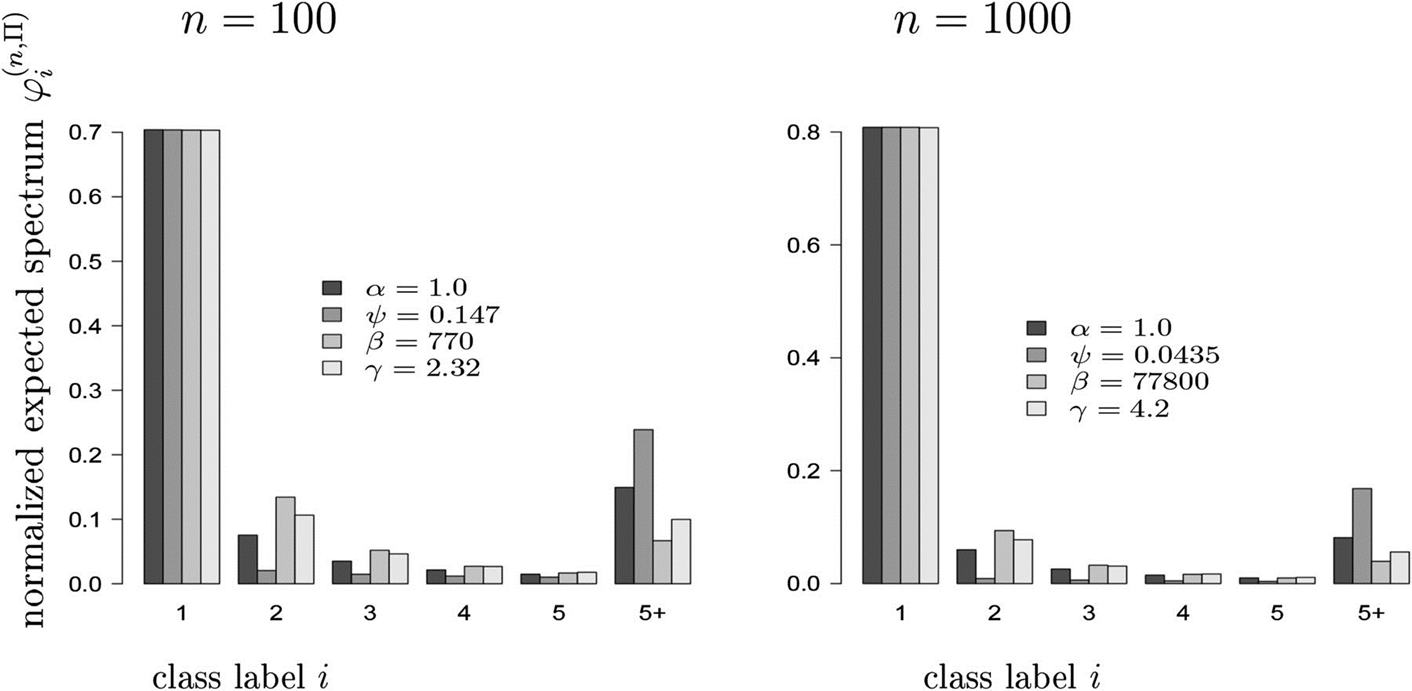
\includegraphics[width=\linewidth]{example-figure}
\caption{Example movie (the figure file above is used as a placeholder for this example). \textit{GENETICS} supports video and movie files that can be linked from any portion of the article - including the abstract. Acceptable formats include .asf, avi, .wav, and all types of Windows Media files.   
}%
\end{figure}


\subsection*{\url Table}

Table \ref{tab:shape-functions} shows an example table. Avoid shading, color type, line drawings, graphics, or other illustrations within tables. Use tables for data only; present drawings, graphics, and illustrations as separate figures. Histograms should not be used to present data that can be captured easily in text or small tables, as they take up much more space.  

Tables numbers are given in Arabic numerals. Tables should not be numbered 1A, 1B, etc., but if necessary, interior parts of the table can be labeled A, B, etc. for easy reference in the text.  


\begin{table*}[htbp]
\centering
\caption{\bf Students and their grades}
\begin{tableminipage}{\textwidth}
\begin{tabularx}{\textwidth}{XXXX}
\hline
Student & Grade\footnote{This is an example of a footnote in a table. Lowercase, superscript italic letters (a, b, c, etc.) are used by default. You can also use *, **, and *** to indicate conventional levels of statistical significance, explained below the table.} & Rank & Notes \\
\hline
Alice & 82\% & 1 & Performed very well.\\
Bob & 65\% & 3 & Not up to his usual standard.\\
Charlie & 73\% & 2 & A good attempt.\\
\hline
\end{tabularx}
  \label{tab:shape-functions}
\end{tableminipage}
\end{table*}


\bibliography{example-bibliography}

\end{document}